% \documentclass[10pt,twocolumn,letterpaper]{article}
\documentclass{article}

 \PassOptionsToPackage{numbers, compress}{natbib}
 
\usepackage{times}
\usepackage{epsfig}
\usepackage{graphicx}
\usepackage{amsmath}
\usepackage{amssymb}
\usepackage{caption}
\usepackage{subcaption}
\usepackage{float}
\usepackage{xcolor}
\usepackage{bbm}
\usepackage{float}

\usepackage[utf8]{inputenc} % allow utf-8 input
\usepackage[T1]{fontenc}    % use 8-bit T1 fonts
\usepackage{hyperref}       % hyperlinks
\usepackage{url}            % simple URL typesetting
\usepackage{booktabs}       % professional-quality tables
\usepackage{amsfonts}       % blackboard math symbols
\usepackage{nicefrac}       % compact symbols for 1/2, etc.
\usepackage{microtype}      % microtypography
\usepackage{xcolor}         % colors


% ready for submission
\usepackage{neurips_2021}

% to compile a preprint version, e.g., for submission to arXiv, add add the
% [preprint] option:
% \usepackage[preprint]{neurips_2021}

% to compile a camera-ready version, add the [final] option, e.g.:
%     \usepackage[final]{neurips_2021}

% to avoid loading the natbib package, add option nonatbib:
%    \usepackage[nonatbib]{neurips_2021}





\newcommand{\R}{\mathbb{R}}
\newcommand{\half}{\frac{1}{2}}
\newcommand{\diag}[1]{\operatorname{diag}\{#1\}}
\newcommand{\red}[1]{\textcolor{red}{#1}}
\newcommand{\blue}[1]{\textcolor{blue}{#1}}
\newcommand{\diff}{\mathrm{d}}
\newcommand{\inner}[2]{\langle #1, #2 \rangle}

\begin{document}


%%%%%%%%% TITLE
\title{ Adaptive Sparse Neighborhood Graph using Quadratically Regularized Optimal Transport }
\red{SZ: might need a more interesting title?}

% \author{Tetsuya Matsumoto, Stephen Zhang, Geoffery Schiebinger \\
% University of British Columbia\\
% Vancouver, B.C., Canada\\
% {\tt\small \{tmats, geoff, syz\}@math.ubc.ca}
% % For a paper whose authors are all at the same institution,
% % omit the following lines up until the closing ``}''.
% % Additional authors and addresses can be added with ``\and'',
% % just like the second author.
% % To save space, use either the email address or home page, not both
% % \and
% % Second Author\\
% % Institution2\\
% % First line of institution2 address\\
% % {\tt\small secondauthor@i2.org}
% }


\author{%
  Dummy \\
%   \thanks{Use footnote for providing further information
    % about author (webpage, alternative address)---\emph{not} for acknowledging
    % funding agencies.} \\
  Department of Mathematics\\
  University of British Columnbia\\
  Vancouver, B.C., Canada \\
  \texttt{@math.ubc.ca} \\
  % examples of more authors
   \And
   Coauthor \\
   Department of Mathematics\\
  University of British Columnbia\\
  Vancouver, B.C., Canada \\
  \texttt{@math.ubc.ca} \\
   \AND
   Coauthor \\
  Department of Mathematics\\
  University of British Columnbia\\
  Vancouver, B.C., Canada \\
  \texttt{@math.ubc.ca} \\
  % \And
  % Coauthor \\
  % Affiliation \\
  % Address \\
  % \texttt{email} \\
  % \And
  % Coauthor \\
  % Affiliation \\
  % Address \\
  % \texttt{email} \\
}


\maketitle

%%%%%%%%% ABSTRACT
\begin{abstract}
   Regularized optimal transport (OT) has been proven to be useful tool in practice due to its computational efficiency and mathematical properties. Often, OT assumes two distributions and a cost function to compute the optimal coupling between the two. In this paper, we propose a method to construct an adaptive sparse neighbourhood graph using optimal transport on a single data. 
\end{abstract}

\begin{figure}[h]
    \centering
    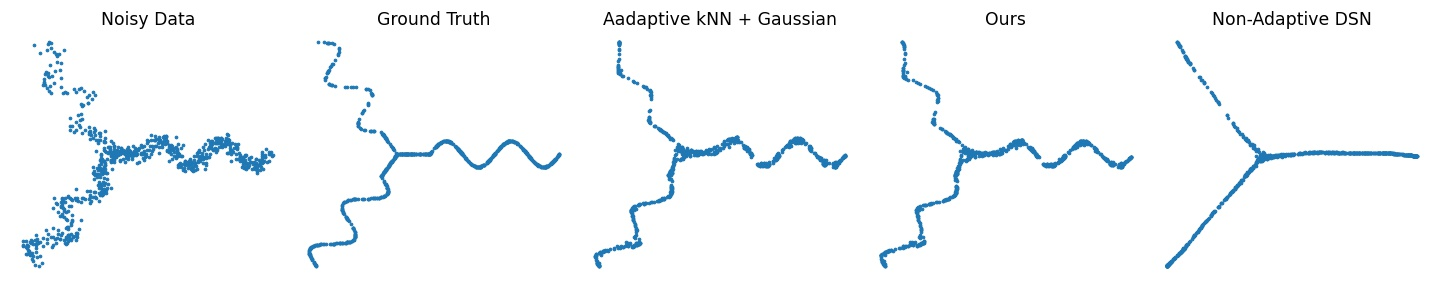
\includegraphics[width=1\textwidth]{LaTeX/figures/ToyMAGIC.jpg}
    \caption{Denoising data using three diffusion operators. Adaptive $k$NN + Gaussian operator \cite{van2018recovering}, ours and non-adaptive doubly-stochastic normalization of Gaussian.}
    \label{fig:ToyMAGIC}
\end{figure}


%%%%%%%%% BODY TEXT
\section{Introduction}

Geometric aspects of datasets play a central role in many machine learning problems. 
Collections of observations are are often represented as sets of points in some space, and the similarity between a pair of observations $(x, y)$ can be measured using a choice of distance or similarity function. 
Tasks such as classification and clustering rely on having relational information between observations, commonly represented as a undirected weighted graph, in which vertices are identified with observations, and edge weights measure the strength of association between observations. 
Many high-dimensional datasets in fact have low-dimensional structure -- i.e. they are comprised of points lying on a low-dimensional manifold embedded within the higher dimensional observation space. This is the well-known \emph{manifold assumption}, which has been observed to hold in many settings such as image and gene expression data \cite{cayton2005algorithms, van2018recovering}. 

The first step of most learning algorithms is to construct a graph modelling relations between observations. Most commonly, a $k$-nearest neighbour ($k$-NN) graph is sought, where each node $x_i$ is assigned edges the $k$ nodes that are closest in the chosen distance $d$. Since $k$-NN membership is not symmetric, this graph is generally directed. However, the graph can be straightforwardly made undirected. Weights are then assigned to the edges typically using an affinity function, i.e. $w_{ij} = f(d(x_i, x_j))$ for $x_i \sim x_j$. One major reason for the widespread use of $k$-NN graphs is that the resulting graphs are \emph{sparse}. This is both a conceptually and computationally desirable property: sparse connections in the graph mean that the $k$-NN model tries to capture relational information in the dataset in a parsimonious way, and sparse matrices enable fast computations on large datasets. 
Another important step is to normalize the weight matrix $w_{ij}$. Normalization of weights plays a prominent role when its spectral properties are concerned. We will discuss different normalization methods and their effects in section \ref{sec:RelatedWork}.

Despite its widespread use, $k$-NN can struggle in settings where the underlying dataset has features on different spatial scales or significant differences in sampling density. 
% \red{Need more discussion of this. Tim?} 
Figure \ref{fig:ToyMAGIC} shows an example of a $k$-NN graph with Gaussian weight function (i.e. $w_{ij} = \exp\left( -d^2(x_i, x_j)/\sigma\right)$) used to denoise data. The reconstructed result fails to capture fine details of wavy arm.
Adaptive approaches have been developed to compensate for variable sample density, in which either $k$ is allowed to vary from observation to observation \cite{balsubramani2019adaptive}, or the width of the affinity function is tuned instead \cite{van2018recovering} (e.g. $\sigma >0$ for Gaussian). However, these methods typically require additional parameters to be chosen \cite{balsubramani2019adaptive, van2018recovering} or some form of density estimation \cite{coifman2005geometric}.

To address this challenge, we introduce a new method to create a neighbourhood graph using Quadratically Regularized Optimal Transport (QROT). 
QROT graph is generated by solving a simple unconstrained optimization problem. This optimization problem has a single parameter to be tuned which acts as the weight bandwidth ($\sigma >0$ in Gaussian) and neighbourhood size ($k$ in $k$-NN) simultaneously. 
This parameter is shown to be more robust to tune, that is, near-optimum performance is achieved in a wide range of the parameter value. 
The motivation for the optimization problem is to obtain a sparse solution while preserving local geometry without relying on a predefined graph such as $k$-NN graph.
However, Gaussian weight function without given locality is necessarily dense and the result is undesirably smoothed. 

We replace the Gaussian kernel by a sparse kernel. The problem of normalizing Gaussian can be performed in the same way on another kernel. One of the normalization technique is Doubly Stochastic Normalization (DSN), also known as matrix scaling problem. DSN of a Gaussian is, in fact, equivalent to solving an Entropically Regularized Optimal Transport (EROT) problem \cite{landa2021doubly} with a special strongly convex cost function. However, DSN of Gaussian cannot straightforwardly be applied with underlying $k$-NN graph structure since the well-known Sinkhorn's algorithm assumes non-zero entries in the weight matrix $w_{ij}$.

In QROT graph method, because we need to consider both sparsity and its spectral property, we evaluate our method on a semi-supervised learning problem and denoising to compare with a classical method by replacing the Gaussian weight matrix with ours. 
These graph-based algorithms are performed based on diffusing according to the kernel on the graph.  
By establishing an adaptive weighted graph, QROT performs better in revealing complex structure in data, such as varying sample density when an adaptive method is required to reconstruct fine details of the data.

In summary, the major contribution of our work is a new OT-based method for weighted neighbourhood graph construction. We have proposed QROT graph method to obtain a sparse, adaptive and doubly stochastic weighted graph on a given dataset. 
Our graph can replace the role of $k$-NN in many applications of weighted $k$-NN graph based methods such as clustering, manifold learning, data denoising, semi-supervised learning, just to name a few.

The rest of the paper is organized as follows. We begin by reviewing classical spectral methods in section \ref{sec:RelatedWork}. The graph construction setup is discussed in section \ref{sec:Method}, followed by a brief formulation of general and regularized OT problems. 
We briefly provide an explanation of why QROT solution is sparse in section \ref{sec:Quadratic}.
Our QROT graph construction is detailed in section \ref{sec:QROTgraph} with its application to Semi-Supervised Learning and cell imputation in section \ref{sec:SSL} and \ref{sec:MAGIC}.
We discuss some limitations and conclusion in section \ref{sec:Discussion}.

\section{Related work}\label{sec:RelatedWork}

Establishing an accurate representation of a dataset is a challenging task in machine learning. Classical weighted graph-based methods are concerned with its spectral property. 
An embedding of a high dimensional dataset into a lower dimensional space is typically described by eigenvectors of so-called graph Laplacian which is induced from the weights on the graph. 
Also, diffusion-based methods on graph is closely related to graph-Laplacian and its eigenvector and eigenvalues which are direct analogue to continuous problems such as Poisson equation and heat equation.

% Given $N$ points $x_1, \ldots, x_N \in \R^N$, let $G=(V, E)$ be the $k$NN graph \red{SZ: I think we should introduce this notational setup earlier in Section 1}. The kernel \blue{matrix} is defined as: 
% \begin{equation}\label{eqn:GraphHeatKernel}
%     K_{ij} = 
%     \begin{cases}
%     e^{-\frac{\|x_i-x_j\|^2}{\sigma^2}} &\text{ if } (x_i, x_j) \in E \\
%     0 &\text{ otherwise.}
%     \end{cases}
% \end{equation}
% with a \blue{bandwidth} parameter $\sigma\in\R$ \blue{that controls how quickly the kernel weight decays as distance between neighbours increases.}
% % The weight matrix $W_{ij} = W(x_i, x_j)$ is 

In spectral methods, weights are assigned to edges of the  $k$-NN graph typically using kernel function such as Gaussian function. 
The weight matrix is given by normalizing the kernel matrix $K_{ij} = k(x_i, x_j)$ with the diagonal degree matrix $D_{ii} = \sum_j K_{ij}.$  There are a number of ways in which this can be done.
\begin{itemize}
    % \item No normalization: \\
    % $W_{\text{un}} = K$
    \item Random walk normalization: 
    $W_{\text{rs}} = D^{-1} K$
    \item Symmetric normalization:
    $W_{\text{sym}} = D^{-\half} K D^{-\half}$
    \item Doubly stochastic normalization:
    $W_{\text{ds}} = \diag{\mathbf{\alpha}} K \diag{\mathbf{\alpha}}$
    \footnote{
    where the vector $\mathbf{\alpha} = (\alpha_1, \ldots, \alpha_N)$ is selected so that $W_{\text{ds}}$ is doubly-stochastic, i.e. every row-sum and column-sum are 1 \cite{landa2021doubly}.}
\end{itemize}

Note that the $W_{\text{rs}}$ and $W_{\text{ds}}$ have the interpretation as being the transition matrix of a Markov chain, since each entry of the matrix is non-negative and sums to 1 along each row by construction.
While $W_{\text{sym}}$ does not have the Markov chain interpretation, it shares the same eigenvectors as $W_{\text{rs}}$ and the symmetry is advantageous in some applications.
Most notably, the doubly-stochastic weight matrix has both stochastic and symmetry properties and it is shown to have robustness to heteroskedastic noise in data \cite{landa2021doubly}.
The key observation is that finding a DSN is, in fact, equivalent to solving an EROT problem which grants us a clear geometric understanding.
However, DSN can only be applied without underlying $k$-NN graph due to its problem formulation and its solver.
We further discuss the doubly-stochastic normalization in section \ref{sec:DSN}.
Looking at the problem from the perspective of OT, we attempt to develop a weighted graph that is also sparse and adaptive.



%-------------------------------------------------------------------------



\section{Method}\label{sec:Method}

In this section, we first introduce basic notations and formulation of OT problem and its regularizations. Importantly, the solution, optimal coupling of a regularized problem is, in fact, a projection of a kernel to the admissible set, which is naturally a normalization of the corresponding kernel. We begin by reviewing the general OT formulation and regularized problems. Then we discuss DSN of Gaussian kernel again and its relation to entropic regularization, which leads us to our graph construction using quadratic regularization.

\subsection{Optimal Transport}\label{sec:OT}
% \red{need general case? redundant?}
\red{SZ: I think you can probably go straight to the regularised case for the purposes of this discussion.}
% \red{SZ: I think also we can just discuss the discrete case? Since we are dealing with kNN}
% Given two probability spaces $(\mathcal{M}, \mathcal{X}, \mu)$ and $(\mathcal{N}, \mathcal{Y}, \nu)$, define
% \begin{equation}\label{eqn:CouplingSpace}
%     \Pi(\mu, \nu) = \left\{ \pi \in \mathcal{M} \times \mathcal{N}: \int \pi(dx, \cdot) = \mu, \int \pi(\cdot, dy) = \nu \right\}
% \end{equation}
% to be the space all coupling between $\mu$ and $\nu.$
% Then, optimal transport solves the following optimization problem:
% \begin{equation}\label{eqn:OTproblem}
%     \min_{\pi \in \Pi(\mu, \nu)} \int C(x, y)  \diff\pi(x, y)
% \end{equation}
% where $C:\mathcal{X}\times\mathcal{Y}\to\R$ is the cost function.

OT problem seeks an assignment of one given probability measure to another, minimizing the cost between the two measures. 
Let $\mu$ be discrete measure on $\mathcal{X} = \R^n$, and $\nu$ another measure on $\mathcal{Y} = \R^m$ and $c:\mathcal{X} \times \mathcal{Y} \to \R,$
(i.e. $\mu = \sum_{i=1}^m \mu_i\delta_{x_i}$ and $\nu = \sum_{j=1}^n \nu_j\delta_{y_j} $ s.t. $\mu_i, \nu_j \ge 0$ and $\sum_i \mu_i = \sum_j\nu_j =1$). 
The \textit{Kantorovich problem} seeks a coupling $\pi^*$ such that:

\begin{equation}\label{eqn:OTproblem}
    \min_{P\in U(\mu, \nu)} \sum_{i, j} c_{i j} \pi_{i j} = \min_{\pi\in U(\mu, \nu)} \langle c, \pi \rangle
\end{equation}
where $c_{ij} = c(x_i, y_j)$ and
\begin{equation}\label{eqn:discreteCouplingSpace}
    U(\mu, \nu) = \left\{\pi\in\R_+^{m\times n} : \sum_j \pi_{i j} = \mu_i,  \sum_i \pi_{i j} = \nu_j \right\}
\end{equation}

While there is a number of methods to solve the linear programming problem \eqref{eqn:OTproblem}, the algorithms can be quite complex and computationally expensive.
However, the optimization problem \eqref{eqn:OTproblem} can be regularized by adding an extra regularization term to approximate the true solution.  
The regularized problem also enjoys several advantages;
it can be written as a simple alternate minimization in the dual form, which results in more efficient and stable numerical algorithm such as well-known \textit{Sinkhorn's algorithm} for entropic regularization \cite{peyre2019computational}.

\subsection{Entropic Regularization}\label{sec:Entropic}

The discrete entropy of a coupling matrix is defined as
\begin{equation}\label{eqn:DiscreteEntropy}
    H(\pi) = -\sum_{i,j} \pi_{i j}\left( \log \pi_{ij} -1 \right)
\end{equation}
(with the convention $H (\pi) = \infty$ if $ \pi_{ij} = 0$ for some pair $(i j)$). 

The entropic regularized optimal transport problem is
\begin{equation}\label{eqn:EntOT}
    \min_{P\in U(\mu, \nu)} \langle c, \pi \rangle - \sigma^2 H(\pi)
\end{equation}
with some $\sigma^2>0.$ 
Since the negative entropy is a 1-strongly convex function, \eqref{eqn:EntOT} has a unique solution. 
Note that the solution to \eqref{eqn:EntOT} converges to the solution of \ref{eqn:OTproblem} in the limit $\sigma^2\to 0$.
Intuitively, the entries of $\pi^*_\sigma$ concentrates near the true solution $\pi^*$ to \eqref{eqn:OTproblem} as $\sigma^2$ decreases to 0.

The entropic regularized problem can also be understood as a projection of Gaussian kernel.
A solution to \eqref{eqn:EntOT}$, \pi_\sigma^*$, is a projection of the Gibbs kernel $G_{i j} = e^{-\frac{c_{i j}}{\sigma^2}}$ onto the admissible coupling set $U(\mu, \nu)$.

More precisely, 
\begin{equation}\label{eqn:KLproj}
    \pi_\sigma^* = \mathop{\mathrm{argmin}}_{\pi\in U(\mu, \nu)} \operatorname{KL}(\pi|G)
\end{equation}
where
\begin{equation}\label{eqn:KLdiv}
    \operatorname{KL}(\pi|G) = \sum_{i, j} \pi_{i j} \log\frac{\pi_{i j}}{G_{i j}} - \pi_{i j} + G_{i j}.
\end{equation}

The discrete entropic problem \eqref{eqn:EntOT} has aforementioned \textit{Sinkhorn's algorithm} to efficiently compute the solution, 
which allows one to write in the form:
\begin{equation}\label{eqn:SinkhornSol}
    \pi_\sigma^* = \diag{\alpha} G \diag{\beta}
\end{equation}
where $(\alpha, \beta) \in \R^n_+\times\R^m_+$ such that 
\begin{equation}
    \diag{\alpha} G \diag{\beta}\mathbbm{1}_{m} = \mu
    \quad\text{ and }\quad
    \diag{\beta} G^T \diag{\alpha}\mathbbm{1}_{n} = \nu
\end{equation}
This condition guarantees that $\pi_\sigma^*\in U(\mu, \nu)$. 
Finding a matrix decomposition of this form is also known as \textit{matrix scaling problem}. 
The Sinkhorn's algorithm iteratively updates $\alpha$ and $\beta$ until convergence. 
% \red{more details about Sinkhorn?}
Each iteration only uses entry-wise matrix division and hence can be computed extremely efficiently on GPU \cite{peyre2019computational}. 



\subsection{Quadratic Regularization of Optimal Transport}\label{sec:Quadratic}

The regularized OT problem is well-defined with any strictly convex refularizer. 
Quadratic regularization of optimal transport (QROT) problem \eqref{eqn:OTproblem} replaces the entropy term of \eqref{eqn:EntOT} by squared norm:
\begin{equation}\label{eqn:QuadOT}
    \min_{\pi\in U(\mu, \nu)} \langle c, \pi \rangle + \frac{\varepsilon}{2} \|\pi\|^2_2
\end{equation}
with $\varepsilon>0.$
The solution to \eqref{eqn:QuadOT} has been known to be a sparse approximation to the true solution, which is a major advantage over the entropic regularization.
However, the Sinkhorn's algorithm does not apply to the QROT problem since it advantage of multiplicative form of dual problem of \eqref{eqn:EntOT}. 
Although quadratic regularization can be written as an alternate minimization problem \cite{lorenz2021quadratically}, each step is not a straightforward matrix multiplication unlike entropic case. 
In this work, we employ semi-smooth Newton's method proposed by Lorentz et al. \cite{lorenz2021quadratically} for our computation. 
% \red{discus more on Lorenz paper?}

QROT problem generally has sparse solution but it is rarely discussed why it tends to be sparse. 
Here, we show that the optimal coupling of \eqref{eqn:QuadOT} is, indeed, the sparsest approximate to the unregularized problem \eqref{eqn:OTproblem} in the L2 sense. 
Dessein et al (2018)\cite{dessein2018regularized} showed that the relation \eqref{eqn:KLproj} holds more generally with any continuously differentiable convex regularizer $\phi$.
That is 
\begin{align}\label{eqn:BregProj}
    \boldsymbol{\pi}_{\lambda}^* 
    &= \underset{\boldsymbol{\pi} \in \Pi(\mu, \nu)}{\operatorname{argmin}}\langle\boldsymbol{\pi}, \boldsymbol{\gamma}\rangle+\lambda \phi(\boldsymbol{\pi})\\
    &= \underset{\boldsymbol{\pi} \in \Pi(\mu, \nu)}{\operatorname{argmin}} B_{\phi}(\boldsymbol{\pi} \| \boldsymbol{\xi})
\end{align}
where $\lambda>0$ and $\xi$ is the global minimizer of $\phi.$
When $\phi(\boldsymbol{\pi}) = \half\|\boldsymbol{\pi}\|^2,$ trivially it has minimizer $\boldsymbol{\xi} = 0$. Thus
\begin{align}
    \boldsymbol{\pi}_{\lambda}^* 
    &= \underset{\boldsymbol{\pi} \in \Pi(\mu, \nu)}{\operatorname{argmin}} B_{\phi}(\boldsymbol{\pi} \| 0)\\
    &= \underset{\boldsymbol{\pi} \in \Pi(\mu, \nu)}{\operatorname{argmin}} \half\|\boldsymbol{\pi}\|^2.
\end{align}
This shows $\boldsymbol{\pi^*_\lambda}$ approximates 0 while remaining in $\Pi(\mu, \nu).$



\subsection{Doubly-Stochastic Normalization (DSN) }\label{sec:DSN}

% \red{is this still a related work? SZ: this corresponds to the case with entropic regularisation, right? Probably worth discussing. In particular highlight the difference between using a quadratic regularisation? }

Let us recall that the doubly-stochastic normalized Gaussian kernel is of the form $W_{\text{rs}} = \diag{\mathbf{\alpha}} K \diag{\mathbf{\alpha}}$ and notice the similarity to \eqref{eqn:SinkhornSol}. 
Indeed, finding the vector $\alpha$ in doubly-stochastic is a matrix scaling problem and can be solved by Sinkhorn's algorithm with one extra constraint that is $\pi_{i i} = 0$.
\begin{align}\label{eqn:DoublyStochastic}
    & \min_{W\in\R^{n\times n}} \sum_{ij} \|x_i - x_j\|^2 W_{ij} - H(W) \\
    & s.t. \quad W \mathbbm{1}_{n}  = W^T \mathbbm{1}_{n} = \mathbbm{1}_{n} , W_{ii} = 0
\end{align}
which is equivalent to \eqref{eqn:EntOT} with special cost function
\begin{equation}\label{eqn:SpecialCost}
    c(x, y) = 
    \begin{cases}
    \infty &\text{ if } x = y\\
    \half\|x-y\|^2 &\text{ otherwise}
    \end{cases}
\end{equation}
and $\mu_i = \nu_i = 1$ for all $i.$
% \red{justify $c(x, y) = \infty$ when $x=y$.} \red{SZ: to be honest I'm still not entirely convinced one needs $C = +\infty$ on the diagonal. The regularisation term should already push the solution away from Id.}
In the original work by Landa et al. \cite{landa2021doubly}, this connection to OT was pointed and given a simple interpretation for the optimal coupling. Each point $x_i$ has unit mass redistribute to other points, minimizing the transportation cost. 
At the same time, each point also receives unit mass from other points by the same amount.
Hence, the entry $W_{ij}$ describes the amount of mass transported from point $x_i$ to $x_j$ and therefore is symmetric and doubly-stochastic. 

% \red{add more analysis }
% Its statistical robustness to noise has been intensely studied. 



\subsection{Our QROT Graph Construction}\label{sec:QROTgraph}

Our graph construction is inspired by the OT interpretation of DSN Gaussian. 
By replacing the entropic regularization term by quadratic term, the sparse nature of QROT problem generates a sparse normalized weight matrix in the same manner.
The graph structure and its weight is determined \textit{simultaneously} as a result of our optimization problem, unlike many popular $k$NN + Gaussian methods in literature.

We construct our sparse neighborhood graph as follows:
For $X = \{x_1, x_2, \ldots, x_N\}$ and $\mu = \frac{1}{N} \sum_i \delta_{x_i}$, solve
\begin{equation}\label{eqn:OurProblem}
    \min_{\pi \in \Pi(\mu,\mu)} \langle c , \pi \rangle + \frac{\varepsilon}{2} \|\pi\|^2
\end{equation}

with cost function 
\begin{equation}\label{eqn:OurCost}
    c(x, y) =
    \begin{cases}
        \half\|x-y\|^2 & \text{ if } x\neq y \\
        \infty  & \text{ if } x = y.
    \end{cases}
\end{equation}

This cost function is of the form $c(x, y) = h(\|x-y\|)$ with 
% $h(r) = \begin{cases}
%     \half r^2 \text{ if } r>0 \\
%     \infty \text{ otherwise.}
% \end{cases}$ 
$h(r) = \half r^2$ if $r>0$ and $h(0)=\infty$ is a strictly convex function.
OT problems with this form of cost functions are known to have unique solution \cite{cavalletti2015existence}. 
With usual quadratic cost $c(x, y) = \half\|x-y\|^2$ and no regularizer, \eqref{eqn:OurProblem} has a trivial solution which is identity. 
By using our special cost function, we obtain a nontrivial coupling that approximates identity. 
Our graph simply takes the optimal solution $\pi^*$ to \eqref{eqn:OurProblem} as the adjacency/weight matrix of the graph. 

This construction has several advantages.
Our QROT graph enjoys all the aforementioned properties of doubly stochastic normalization of Gaussian weight matrix. 
Namely, it is symmetric, doubly stochastic, has the same simple interpretation. 
But unlike DSN of Gaussian, equivalently entropic regularization, the optimal coupling of quadratic regularization is sparse. 
The sparse property is particularly useful when defining a graph in this manner as DSN does not use incorporate underlying neighbourhood structure such as popular $k$NN structure in classical normalization of Gaussian, which necessarily makes DSN graph dense. 
Further, we claim the graph defined by $\pi^*$ is \textit{adaptive} to its domain. 
One of disadvantages of $k$NN method is that it is crucial to choose $k$ or adapt $k$ in data when the sampling density varies. 
The performance of $k$NN methods rely heavily on the choice of $k.$
Often, one needs to change the value of $k$ and Gaussian parameter $\sigma>0$ by the sample size $N$ and it requires cross validation to determine effective parameters.
Our QROT graph is robust to choice of parameter $\varepsilon>0,$ i.e. it performs close to optimal in wide range of $\varepsilon.$

\blue{There are some adaptive $k$NN methods in literature which attempts to use different $k$ based on local density (CITE) or Gaussian parameter $\sigma$ (CITE).
However, these algorithm suffers from extra computational complexity and robustness \red{NEED MORE STUDY}.
Our QROT graph is completely independent of predefined neighbourhood structure and chooses appropriate number of neighbors and weight simultaneously. 
We show this effect in detail through examples and applications in the next section.
}
\section{Result}

\subsection{Semi-Supervised Learning}\label{sec:SSL}

Semi-Supervised Learning (SSL) predicts unknown labels in the data from a small fraction of labeled data. 
A number of interpretable SSL algorithms employ label propagation by solving a optimization problem through graph-based diffusion according to some diffusion operator on the graph. 
Many of typical choices of the diffusion operator are variants of Gaussian kernel together with underlying $k$NN graph. 
To state the problem more precisely, let us introduce some notations.
Given input data points $X = \{x_1, \ldots, x_N\} \subset \R^D$ stored as a $N\times D$ matrix, define the \textit{label selection matrix} as $N\times N$ diagonal matrix
\begin{equation}
    S_{ii} =  
    \begin{cases}
        1 \quad\text{ if $x_i$ is labeled} \\
        0 \quad\text{otherwise.}
    \end{cases}
\end{equation}
If there are $C$ classes of labels, we construct a $N\times C$ matrix $P$ to store given labels by
\begin{equation}
    P_{ik} = 
    \begin{cases}
        1 \quad \text{if $x_i$ is given label $k$}\\
        0 \quad\text{otherwise.}
    \end{cases}
\end{equation}
Lastly, let $Q$ be the \textit{likelihood score}, the probability of $x_i$ being given label $k$ of $C$ classes which is another $N\times C$ matrix to be optimized. 
Using a weight matrix $W$, or equivalently graph Laplacian $L = I -W$, we solve for $Q$ that minimizes:
\begin{equation}\label{eqn:SSLenergy}
    \min_Q \|SQ-P\|_F^2 + \eta\operatorname{Tr}\left(Q^T L Q\right)
\end{equation}
with $\eta>0.$
Minimizing the first term in \eqref{eqn:SSLenergy} promotes $Q$ to preserve known labels stored as $P.$
In other words, it is a softened constrain instead of a hard constrain forcing $SQ = P$ to preserve exact known labels.
The second term can also be written as $\sum W_{ij} \|Q_i - Q_j\|^2$ if the weight is normalized. 
Minimizing amounts to a smooth assignment of labels onto unknown labels according to the Weight.
Indeed, it is an implicit integration step of diffusion [CITE?].
Since \eqref{eqn:SSLenergy} is an unconstrained convex optimization problem, differentiating the objective function reduces to solving a simple linear equation:
\begin{equation}\label{eqn:SSLeqn}
    \left(S + \eta L\right) Q = P.
\end{equation}
It is worth noting that since $\left(S + \eta L\right)$ is positive (semi-) definite and if the weight matrix is sparse, we may use a sparse linear solver to find the solution to \eqref{eqn:SSLeqn} efficiently. 
We evaluate our QROT graph against $k$NN graph with Gaussian weights by performing SSL solving \eqref{eqn:SSLeqn} on 10-spiral synthetic data.
Each arm is parametrized by $t\in (0.5, 5)$ (so that $t=0$ is at the centre of the spiral) (Figure  \ref{fig:Inferred}). 

\begin{figure}[H]
    \centering
    \begin{subfigure}{0.3\textwidth}
        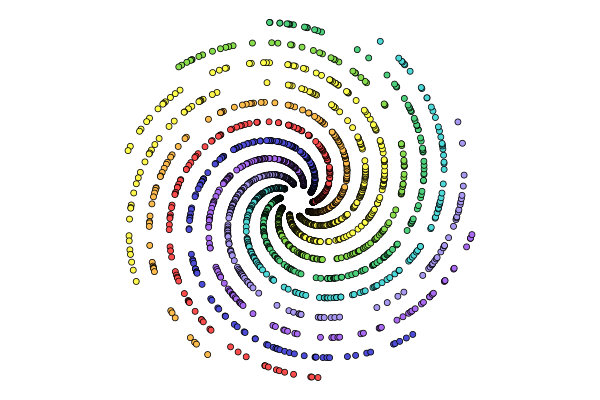
\includegraphics[width=\textwidth]{LaTeX/figures/SpiralData.png}
        \caption{Input Data}
    \end{subfigure}
    \begin{subfigure}{0.3\textwidth}
    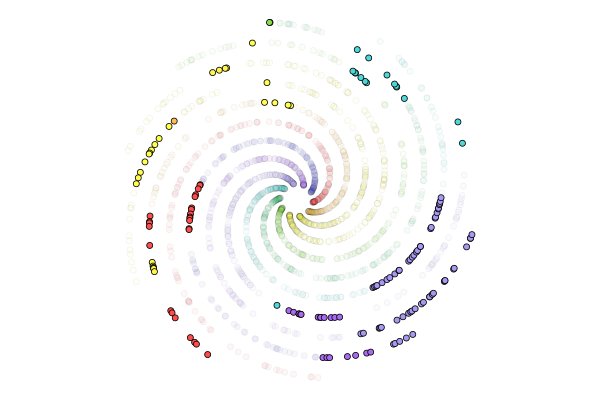
\includegraphics[width=\textwidth]{LaTeX/figures/QOT_infered925.png}
    \caption{Our QROT graph}
    \end{subfigure}
    \begin{subfigure}{0.3\textwidth}
    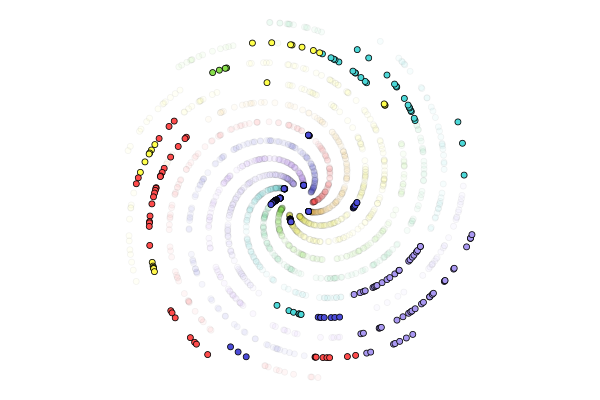
\includegraphics[width=\textwidth]{LaTeX/figures/KNN_infered857.png}
    \caption{$k$NN + Gaussian}
    \end{subfigure}
    \caption{SSL result with 10\% given labels. Each arm of the spiral has 200 points. (a) accuracy = 91.7\% with $\varepsilon=1.0$, (b) accuracy = 86.5\% with $k$ = 5, $\sigma$ = 1.0.}
    \label{fig:Inferred}
\end{figure}

$k$NN methods in general can suffer when the dataset has varying sampling density, requiring to use adaptive $k$ depending on local density of sample points. 
The synthetic spiral data has higher density near the centre and lower density away from the centre. 
To see the adaptivity of our graph, we compare the accuracy along each arm.
Figure \ref{fig:t_vs_param} shows our QROT graph attains higher accuracy over wide range of parameter $\varepsilon$ compared to $k$NN graph.
The optimal $k$ is between 4 to 10 while optimal $\varepsilon$ takes value in $(-0.5, 0.5)$ on the $\log$ domain.
 
\begin{figure}[H]
    \centering
    \begin{subfigure}{0.45\textwidth}
    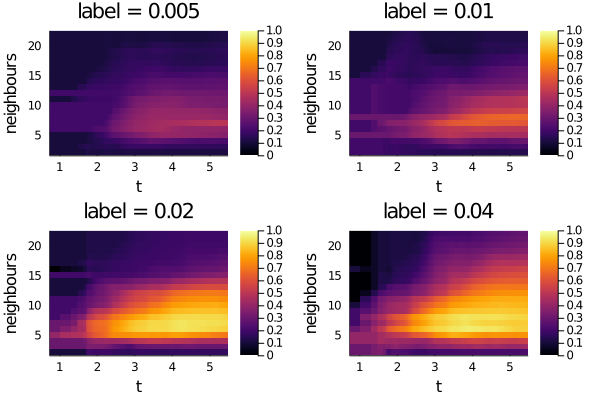
\includegraphics[width=\textwidth]{LaTeX/figures/KNN_unf4.png}
    \caption{kNN + Gaussian}
    \end{subfigure}
    \begin{subfigure}{0.45\textwidth}
    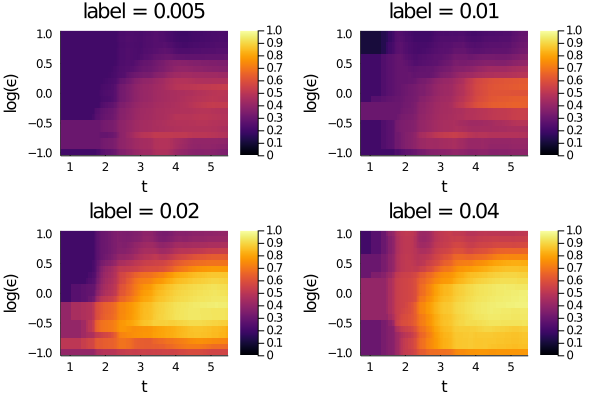
\includegraphics[width=\textwidth]{LaTeX/figures/QOT_unf4.png}
    \caption{our QOT graph}
    \end{subfigure}
    \caption{Heatmap of averaged accuracy over 10 arms of 200 points with four given label proportions. $x$ axis is the parameter $t$ along each arm. $y$ axis is the parameter of each method. }
    \label{fig:t_vs_param}
\end{figure}

The dependence on local sampling density also means it requires to use different $k$ value as local sampling density also changes. 
In practice, the optimal $k$ needs to be determined through cross validation.
In Figure \ref{fig:arm_vs_param} (a), the optimal $k$ increases from 5 to 15 as the density along each arm increases.
While $k$NN suffers from sampling density, our QROT graph has optimal $\varepsilon$ around 0 on the $\log$ domain in all cases. 

\begin{figure}[H]
    \centering
    \begin{subfigure}{0.45\textwidth}
    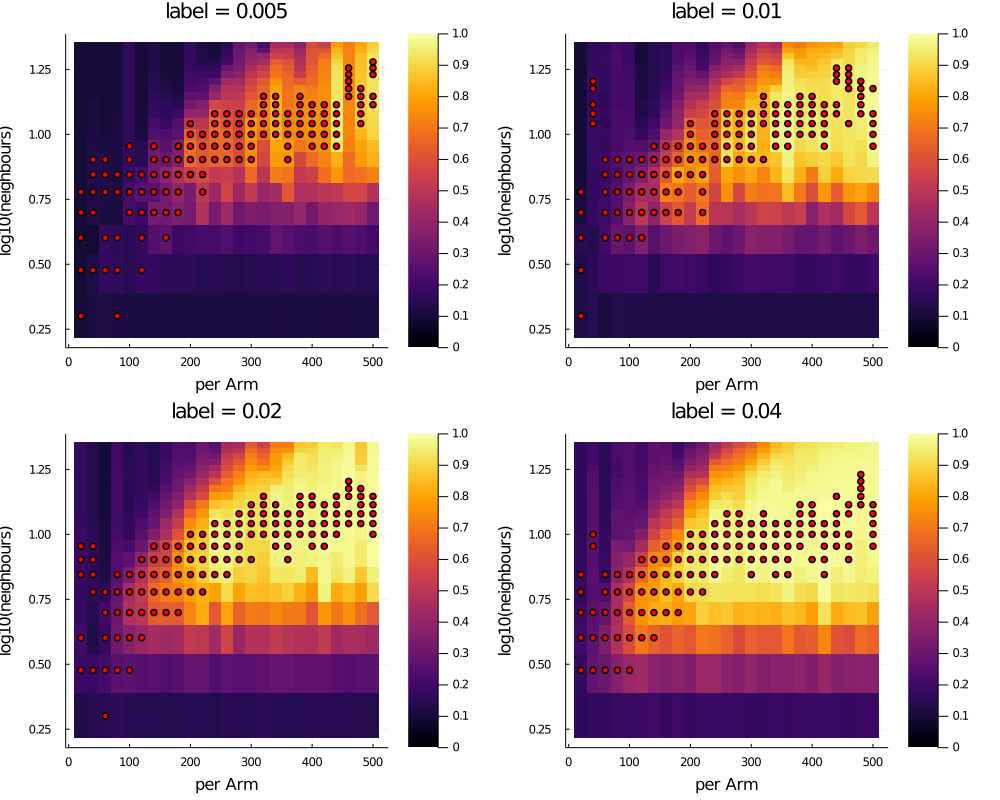
\includegraphics[width=\textwidth]{LaTeX/figures/KNN_max5.png}
    \caption{kNN + Gaussian}
    \end{subfigure}
    \begin{subfigure}{0.45\textwidth}
    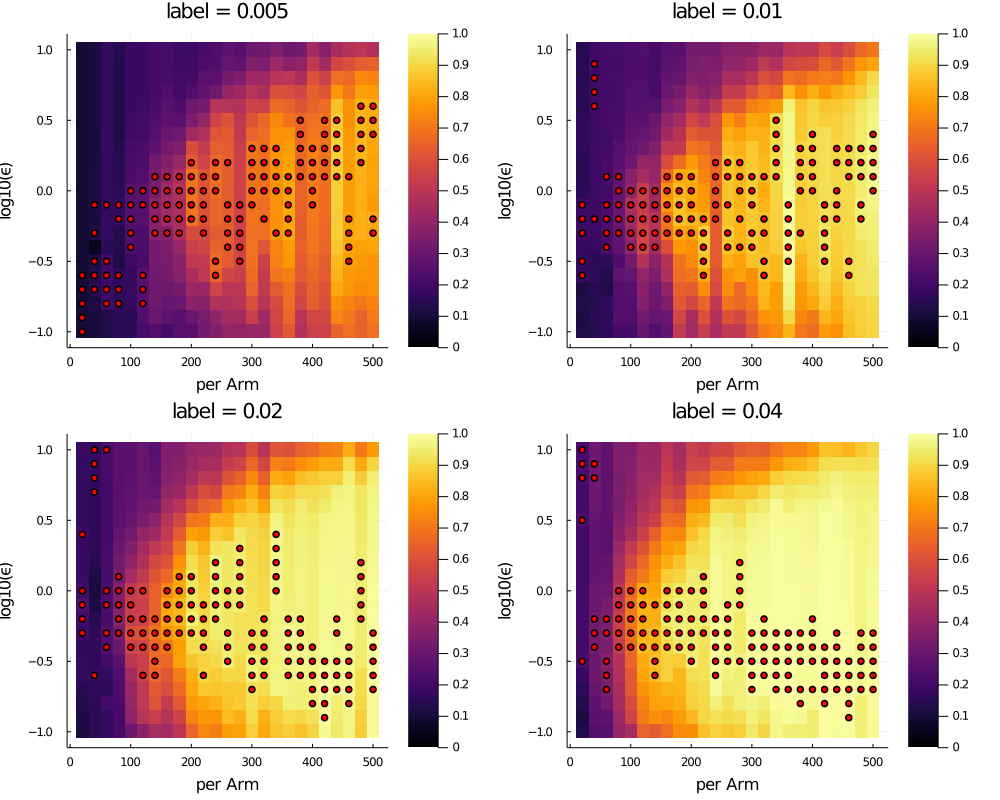
\includegraphics[width=\textwidth]{LaTeX/figures/QOT_max5.png}
    \caption{our QROT graph}
    \end{subfigure}
    \caption{Heatmap of accuracy, number of points per arm vs parameter with four given label proportions. The line plots are the best 5 parameter values for each number of points per arm.}
    \label{fig:arm_vs_param}
\end{figure}

Figure \ref{fig:QOT_KNN_Best} compares the performance of QROT and $k$NN graphs with optimal parameter and best fixed parameter. 
When parameters are tuned, both methods perform at similar capacity in all cases.
The difference starts to show when the parameter is fixed; $k$NN noticeably falls behind with number of points per arm less than 250. 
On the contrary, our QOT with fixed parameter $\varepsilon = 1.0$ performs near optimum in all cases.
% This indicates the QROT graph is \textit{adapting} to the data

\begin{figure}[h]
    \centering
    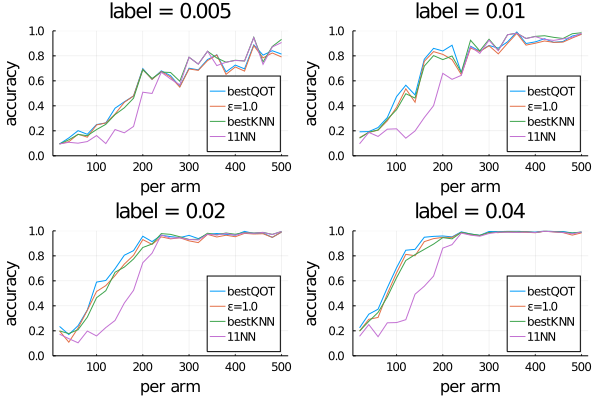
\includegraphics[width=0.6\textwidth]{LaTeX/figures/QOT10_KNNbest.png}
    \caption{Accuracy of SSL result using $k$-NN and QROT graph. The data set is 10-arm spiral with varying number of points per arm.}
    \label{fig:QOT_KNN_Best}
\end{figure}

Variants of graph-based SSL algorithms involve adding more constraints on the optimization to force certain properties such as symmetry, positivity and normalization \cite{wang2007label}. 
Karasuyama and Mamitsuka \cite{karasuyama2017adaptive} proposed an adaptive method by optimizing the $D$ scaling Gaussian parameter $\sigma = (\sigma_1, \ldots, \sigma_D)$; however, their optimization problem becomes nonconvex which can be expensive to solve with higher dimensional input data.

Budninsliy et al. \cite{budninskiy2020laplacian} introduces bi-convex alternating minimization scheme to optimize their Laplacian and likelihood $Q$, motivated by discrete differential geometry. 
This formulation requires to iteratively optimize the Laplacian and $Q$ matrix. 
In particular, optimizing the Laplacian leads to a quadratic programming problem which uses Entropic Mirror Descent to solve. 
In practice, this solver can be numerically unstable and needs extra hyper parameter to be tuned in order for it to update weights properly. 

\subsection{Application to Cell Imputation}\label{sec:MAGIC}

Single-cell RNA sequencing data suffers from many sources of noise, which makes the analysis of gene-gene relationship difficult. 
To address this problem, denoising algorithm using graph-based diffusion algorithms are proposed. 
MAGIC (Markov affinity-based graph imputation of cells) developed by Van et al. \cite{van2018recovering} uses an adaptive Gaussian kernel to impute the data. 
For each point $x_i$ in the data, the Gaussian parameter $\sigma_i$ is chosen by $\sigma_i = d(x_i, x^j_i)$ where $x^j_i$ is the $j$-th nearest neighbour of $x_i.$
This allows the kernel to have larger bandwidth in sparse area and smaller in dense area.

MAGIC computes the diffusion operator by taking the matrix exponent of a given normalized weight matrix $W$ and apply to the data matrix as a smoothing operator. 
% For details, see \cite{van2018recovering}.
As in \ref{fig:ToyMAGIC}, using an adaptive kernel in MAGIC significantly influences the performance. 
In Figure \ref{fig:cellMAGIC}, we compared results after imputation using three kernels.  


\begin{figure}[h!]
    \centering
    \begin{subfigure}{0.25\textwidth}
    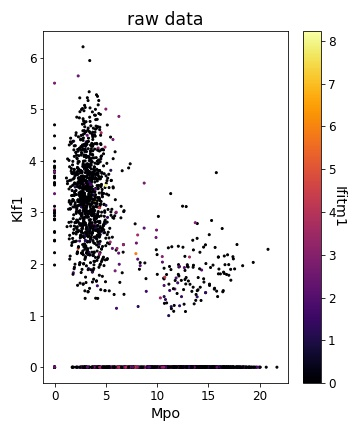
\includegraphics[width=\textwidth]{LaTeX/figures/MAGICdata.jpg}
    \caption{Raw Data}
    \end{subfigure}
    \begin{subfigure}{0.9\textwidth}
    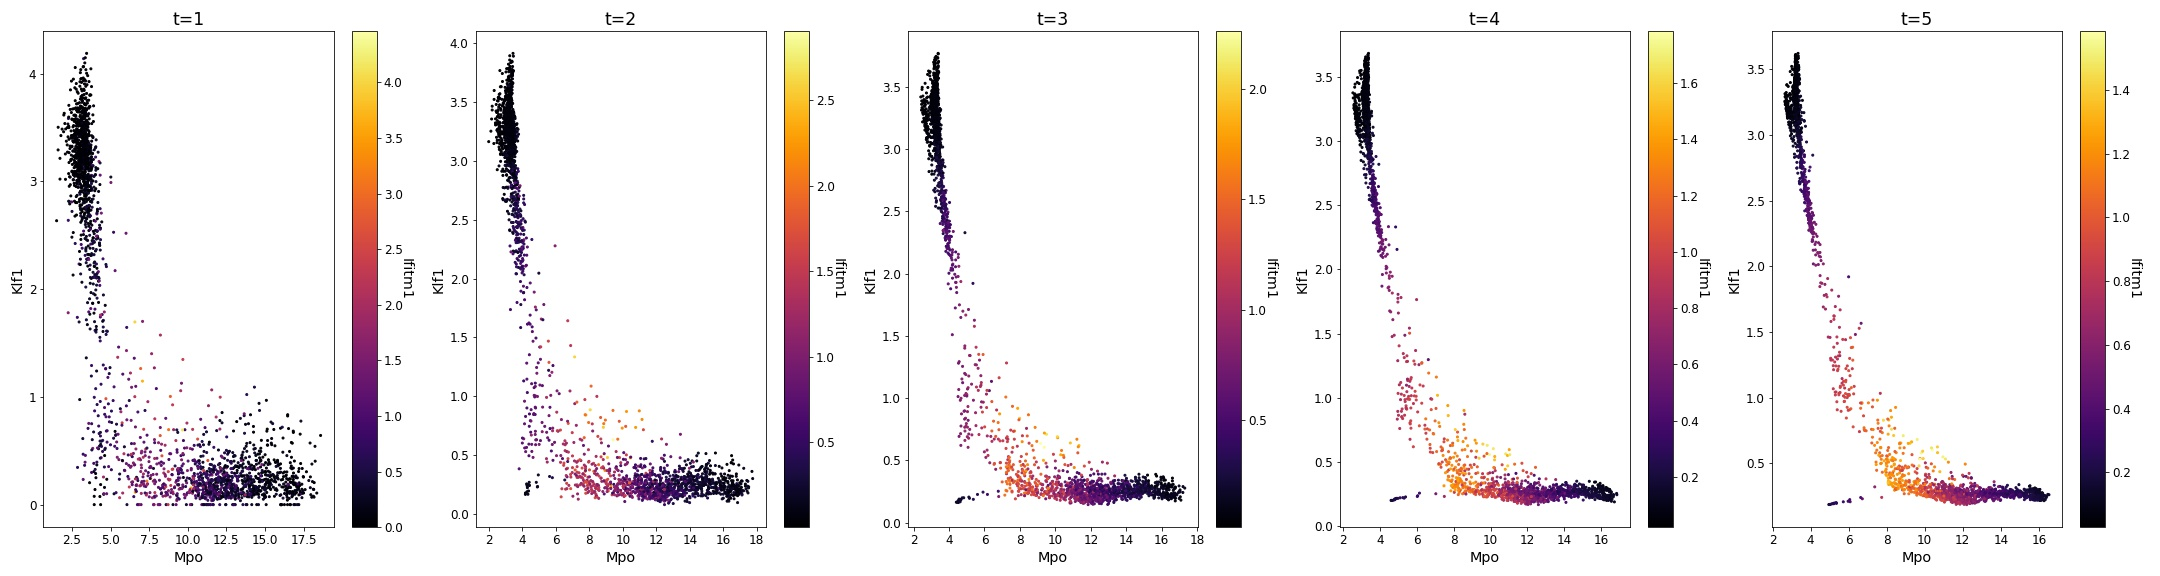
\includegraphics[width=\textwidth]{LaTeX/figures/ORG_MAGIC.jpg}
    \caption{Original MAGIC}
    \end{subfigure}
    \begin{subfigure}{0.9\textwidth}
    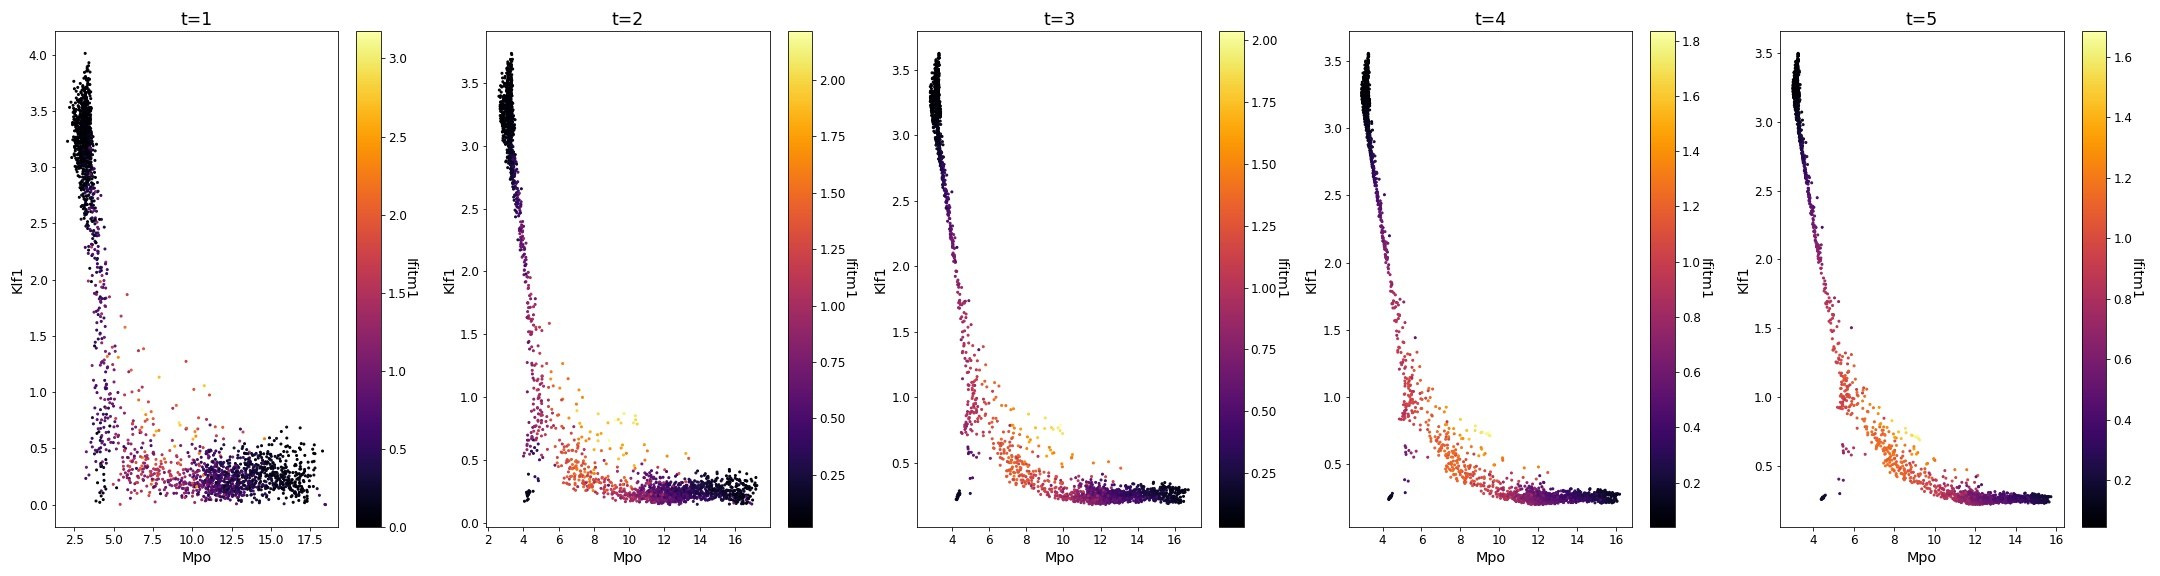
\includegraphics[width=\textwidth]{LaTeX/figures/QOT_MAGIC.jpg}
    \caption{QOT MAGIC}
    \end{subfigure}
    \begin{subfigure}{0.9\textwidth}
    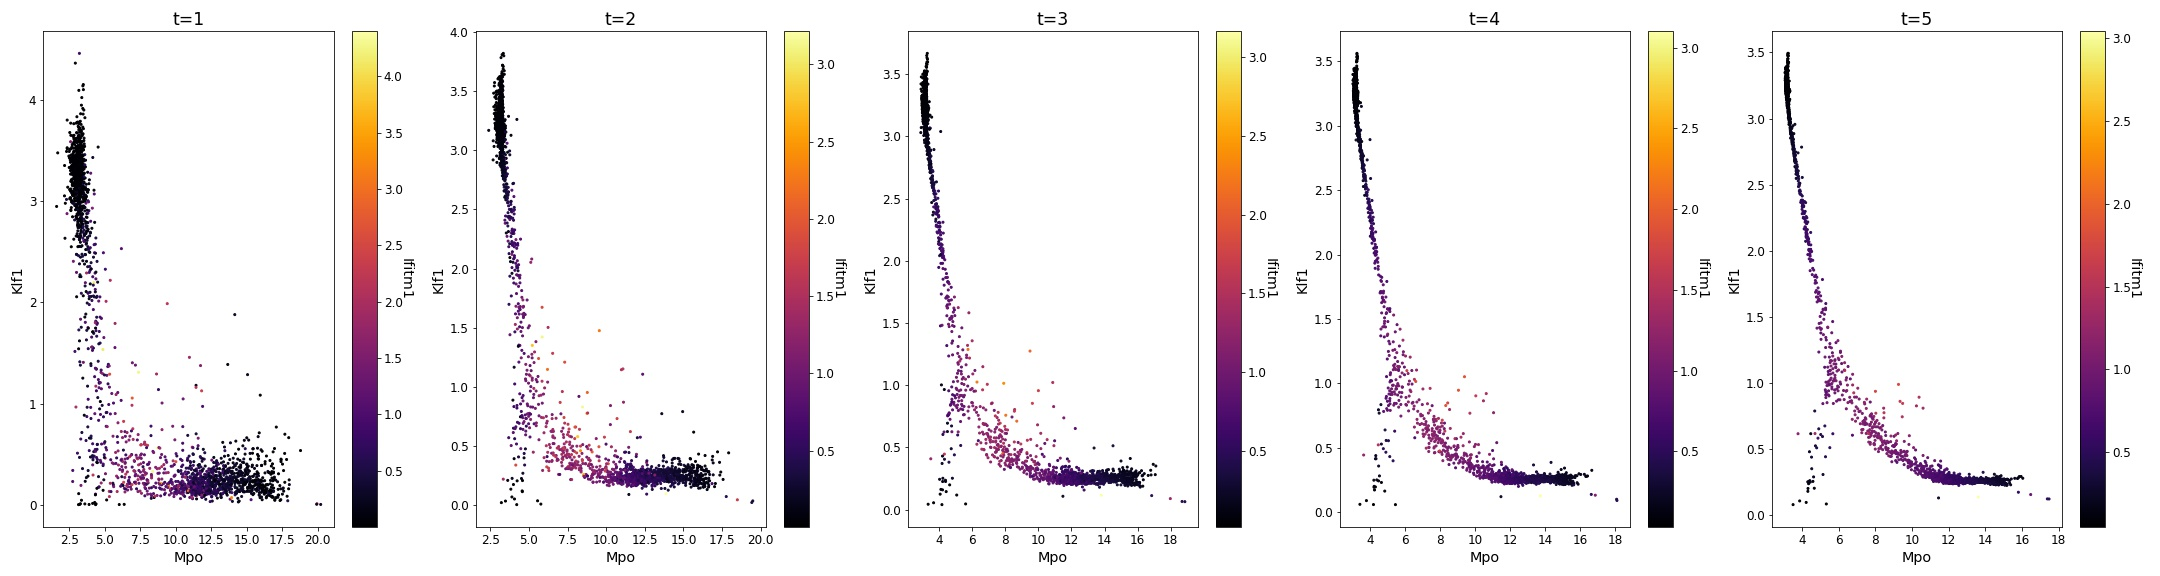
\includegraphics[width=\textwidth]{LaTeX/figures/ENT_MAGIC.jpg}
    \caption{Entropic MAGIC}
    \end{subfigure}
    \caption{Caption}
    \label{fig:cellMAGIC}
\end{figure}


\section{Discussion}\label{sec:Discussion}

The QROT graph is a simple, adaptive method that is applicable to wide range of applications in geometric machine learning tasks where $k$-NN has been traditionally used. It is not only sparse but also adaptive to its domain, which is lacking from $k$-NN based graph methods in general. Our results show that QROT has advantages over classical $k$-NN weighted graph especially when the geometry in data is complicated. The QROT graph can be incorporated into wide variety of applications in data analysis, visualization, processing and more. Its theoretical foundation is simple and solid that complements the weak aspects of every known normalization of Gaussian weight on a graph. 

In future work, it is of interest to study the convergence of our graph Laplacian to the Laplace-Beltrami operator which could suggest a natural connection between theory of OT and geometry. 
% On the practical side, applying the QROT graph in place of well-known machine learning algorithms relying on geometry such as UMAP could be of interest. 
On the practical side, it is important to estimate the best parameter $\varepsilon$ automatically and establish more general understanding of how the optimal coupling $\pi$ is related to the parameter $\varepsilon.$


\newpage

{\small
\bibliographystyle{ieee_fullname}
\bibliography{references.bib}
}

\end{document}
